\clearpage
\section{Procedures}\label{procedures}
Responding to service requests/incidents, generally, is not a simple matter. Service request management and incident management and response activities require knowledge, communication, and coordination among all the people that have to
respond to the service request/incident. Accordingly, the goals of this plan are:
\begin{enumerate}
	\item provides high-quality customer service and results;
	\item responding, systematically, following proven procedures, which will be saving time and money;
	\item minimizing the impact on the interest and honor of \textit{\gls{perc}}.
\end{enumerate}

\subsection{Purpose}\label{purpose}	
This document describes the	overall plan for responding to requests/incidents regarding the e-learning Certified Employee Training Program distributes by \textit{\gls{perc}}. It defines the roles and responsibilities of all the participants with the goal of detecting and react to incidents, determines their scope and risk, responds appropriately to the incident, communicates the results and the risk to all stakeholders, and reduces the likelihood of the incident from reoccurring.

\subsection{Audience}	
  
This plan applies to the call center operators and any person who gains access to SysAid.	
  	
\subsection{Maintenance}  
Giglium is responsible for the maintenance and revision of this document, with the help of \textit{\gls{perc}}.

\subsubsection{Definitions}
The following definitions are used in the next sections:
\begin{itemize}
	\item \textbf{Service request} is a formal request from a user for something to be provided. For example, a request for information or advice.	
	
	\item \textbf{Incidents} is any event that is not part of the standard operation of the \gls{perc} e-learning Certified Employee Training Program service and which causes an interruption or a reduction in quality of the service.
	
	\item \textbf{Workaround} is a temporary fix to an incident or sequence of actions alternative to the one that produces the accident, usable by the final user.
	
	\item \textbf{Personal Information} is the combination of a person’s first name (or initial) and surname, in combination with any of the following:
	\begin{itemize}
		\item social security number;
		\item driver’s license number;
		\item state identification card number;
		\item financial account, debit, or credit number;
	\end{itemize}
\end{itemize}

\subsection{Service Requests Management}
Giglium recommends that service request management have to be managed through a process. This process includes a number of sub-processes that accompany the request from the submission through its closure, where continuous monitoring, tracking, and communication are involved throughout each step. Giglium strongly suggests these sub-processes:
\begin{enumerate}
	\item service request submitted;
	\item service request assessed;
	\item service request fulfilled;
	\item service request closed.
\end{enumerate}

\begin{figure}[h!]
	\centering
	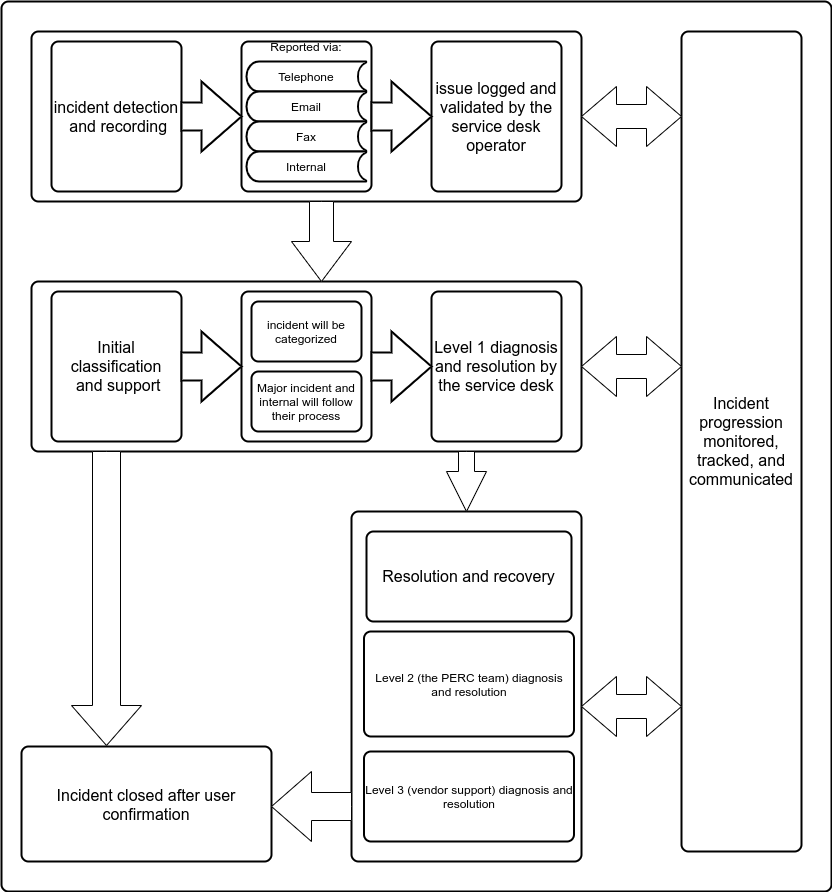
\includegraphics[width=120mm]{./img/procedures/incident-workflow.png}
	\caption{Service request management process}\label{fig:request-wrokflow}
\end{figure}

\subsubsection{Service Request Submitted}
Users can submit a request for service by:
\begin{itemize}
	\item \textbf{Telephone}: the help desk can be notified by calling them at 1 (800) XXXX\footnote{The real telephone number will be defined after the sign of the proposal. But the toll-free number 1 (800) will be preserved.\label{fnlabel}}.
	
	\item \textbf{Email and fax}: the help desk can be notified by sending an email at \href{mailto:info@propanesafety.com}{info@propanesafety.com} or by fax at 1 (800) XXXX\footref{fnlabel}.
\end{itemize}
On the first contact, a ticket is automatically open in the service request section of SysAid.

\subsubsection{Service Request Assessed}
The Help Desk team must first assess the request before any actions are taken to fulfill it. The operator will compile all the fields on the SysAid’s Service Request management triage page to classify the service request. If the information provided by the user isn't enough to fulfill the service request it will ask for more information. During this phase, the operator will assign a priority following the table~\ref{tab:request-priority}.

\begin{table}[H]
	\centering
	\begin{tabular}{ | l | l | l | l | l | }
		\cline{3-5}
		\multicolumn{2}{c|}{}& \multicolumn{3}{|c|}{Impact}  \\ \cline{3-5}
		\multicolumn{2}{c|}{} &Low & Medium  & High \\ \hline
		\multirow{3}{*}{\rotatebox{90}{\tiny Urgency\,}} & Low & \cellcolor{green}Low & \cellcolor{yellow}Medium & \cellcolor{red}High\\ \cline{2-5}
		&   Medium & \cellcolor{yellow}Medium & \cellcolor{yellow}Medium & \cellcolor{red}High \\ \cline{2-5}
		&  High & \cellcolor{red}High & \cellcolor{red}High & \cellcolor{red}High \\ \hline
	\end{tabular}
	\captionof{table}{Service request priority matrix}\label{tab:request-priority}
\end{table}
\gls{perc} and Giglium they expect most requests to be a request for information, concerning:
\begin{itemize}
	\item Installation questions (on individual work stations or across an Intranet);
	\item DVD activation questions (where to find the key code or looking up a missing key code in
	the key code database);
	\item Navigation questions (how to navigate through the interface);
	\item File sharing questions (how to locate and transfer a student record flat file);
	\item General troubleshooting;
	\item questions and issue about the “time bomb”.
\end{itemize}

For this request of information application-specific training and scripts for the operators will be provided by \gls{perc}. They required that the Help Desk personnel will not support the following types of questions, but it will be provided with a script on where to refer users:
\begin{itemize}
	\item Content-related questions;
	\item Identification of Certified Employee Training Program instructors;
	\item Certification/examination issues;
	\item Advanced network-specific questions.
\end{itemize}

Since a request for information doesn't require any planning or approval they are fulfilled during the service request assessed sub-process, from the help desk operator. The operator will simply respond by following the instructions received from \textit{\gls{perc}}, and it will found them inside the SysAid \textit{\gls{kb}}.

\begin{tcolorbox}
	If during the Service request assessed the operator believes that the service request is an incident it has to follow the incident management process describe at~\ref{incident}.
\end{tcolorbox}

\subsubsection{Service Request Fulfilled}
\gls{perc} required that all the requests for service, that are not requesting for information, have to be approved by a supervisor of the related competence area. The operator will put this request in the wait for approval state on SysAid and the system will automatically assign the ticket to the right person, notify it by email. The approver needs to provide a supply list, estimated time for completion, and the instruction so the operator can complete the request satisfactorily.

\subsubsection{Service request closed}
The importance of post-service request fulfillment activities is often underestimated. The ticket is maintained in SysAid since they provide key data such as the overall \textit{\gls{mttr}} tickets and each operator's \textit{\gls{mttr}}. They also contribute to workflow analysis to improve the service request process. The operator will also send a survey to the users who open the request for service to ask for feedback.

\subsubsection{Service Catalog}
Giglium will not implement any service catalog because \textit{\gls{perc}} it will create a comprehensive online service catalog, based on the history of previous service requests registered on SysAid by querying the custom \textit{\gls{api}}~(for \textit{\gls{api}} info see section~\ref{setup}).

\clearpage
\subsection{Incident Management}\label{incident}
Giglium recommends that incidents have to be managed through a process. This process includes a number of sub-processes that accompany the incident from the initial identification or reporting through its resolution and the closure, where continuous monitoring, tracking, and communication are involved throughout each step. Giglium strongly suggests these sub-processes:
\begin{enumerate}
	\item incident detection and recording;
	\item initial classification and support;
	\item investigation and diagnosis;
	\item resolution and recovery;
	\item incident closure.
\end{enumerate}

\begin{figure}[ht!]
	\centering
	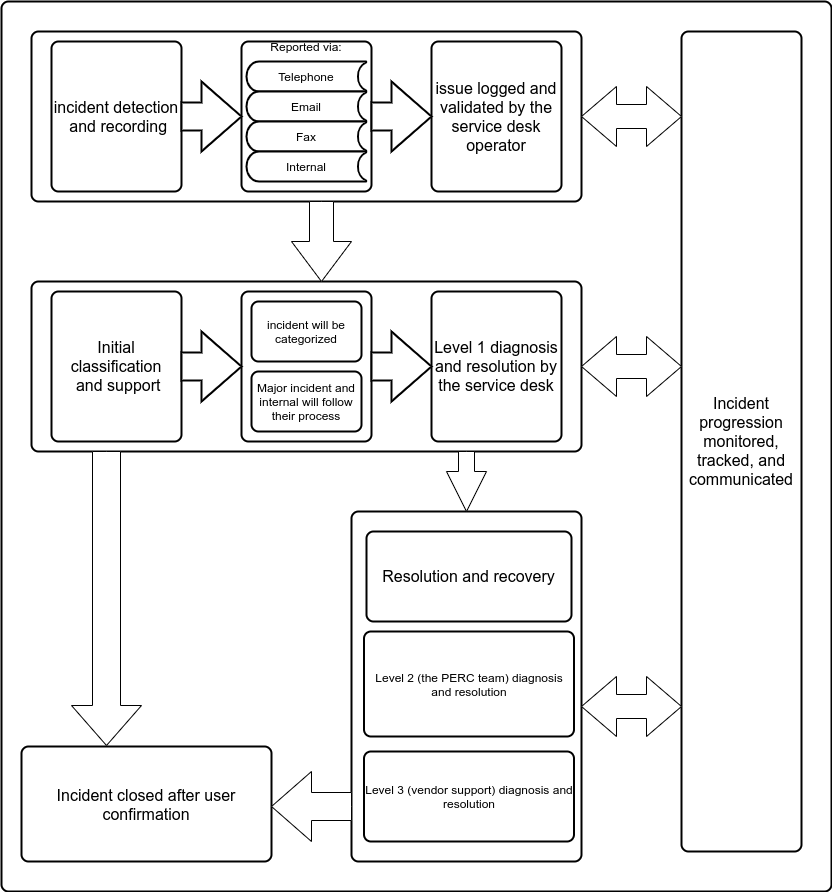
\includegraphics[width=120mm]{./img/procedures/incident-workflow.png}
	\caption{Incident Management Process}\label{fig:incident-wrokflow}
\end{figure}

\subsubsection{Incident detection and recording}
An incident can arrive from the following sources:
\begin{itemize}
	\item \textbf{Telephone, email, and fax}: during the Service request assessed phase if the operator believes that the service request is an incident it will open an incident ticket. The operator will ask the following questions to verify and collect all the information regarding the incident:
	\begin{itemize}
		\item Who is calling? Name and Title?
		\item What is their contact phone number or email address?
		\item What is the DVD key code?
		\item What is the disservice he encounters?
	\end{itemize}
	
	\item \textbf{Internal}: For internal use only. Sometimes the SysAid user can found some incident that impacts his works or the service. In this case, we will track this event with the opening of a ticket and we will process it with a specific workflow. 
\end{itemize}

When a ticket is open in SysAid all the designated party~(s) will be notified.

\begin{tcolorbox}
	It's important to notice that during this initial phase we will collect some users' personal information. It's very important to keep them safe and for this reason, they will be stored only inside the Database and they will be not queryable from any SysAid \textit{\gls{api}}.
\end{tcolorbox}

\subsubsection{Initial classification and support}
The operator will have the SysAid’s Incident Management tool available outlining the necessary information needed for the appropriate response and who should be alerted regarding this incident. The operator will compile all the fields on the SysAid’s Incident Management triage page to classify the incident. During this phase, the operator will assign a priority following the table~\ref{tab:incident-priority}.of the related competence area.


\begin{table}[H]
	\centering
	\begin{tabular}{ | l | l | l | l | l | }
		\cline{3-5}
		\multicolumn{2}{c|}{}& \multicolumn{3}{|c|}{Impact}  \\ \cline{3-5}
		\multicolumn{2}{c|}{} &Low & Medium  & High \\ \hline
		\multirow{3}{*}{\rotatebox{90}{\tiny Urgency\,}} & Low & \cellcolor{green}Low & \cellcolor{yellow}Medium & \cellcolor{red}High\\ \cline{2-5}
		&   Medium & \cellcolor{yellow}Medium & \cellcolor{yellow}Medium & \cellcolor{red}High \\ \cline{2-5}
		&  High & \cellcolor{red}High & \cellcolor{red}High & \cellcolor{red}High \\ \hline
	\end{tabular}
	\captionof{table}{Incident priority matrix}\label{tab:incident-priority}
\end{table}

The operator will perform an initial diagnosis and, it will consult the \textit{\gls{kb}}, to find possible incident resolution tips and how-to solutions. The scope of this initial diagnosis is to provide a workaround for the impacted user. There are two use cases that don't require any diagnosis and need to be immediately escalated:

\begin{itemize}
	\item in case of major incident \textit{\gls{perc}} required to escalate the issue to its dedicated team of experts, of the related competence area. For this reason, the operator will not perform any diagnosis and the related ticket of the incident will be assigned to the on-call person of that area. If the major incident is reported via telephone the call will be redirected to the designated on-call person; 
	\item in case of internal incident Giglium required to escalate the issue to its dedicated \textit{\gls{msp}} team. For this reason, the operator will not perform any diagnosis and the related ticket of the incident will be assigned to the on-call person. 
\end{itemize}

\subsubsection{Investigation and diagnosis}
Giglium will not detail a lot this sub-process since is a \textit{\gls{perc}} responsibility but, after an initial assessment of an incident, the ticket is assigned to the \textit{\gls{perc}} team. The scope of this team is to collect additional information and analyzed them to definitively eliminate the possible cause. In this sub-process, it can be involved even external vendors. This requires a detailed recording of the actions taken and the corresponding results. 
Giglium will keep the responsibility of the communication with all the designated party~(s).

\subsubsection{Resolution and recovery}
When the \textit{\gls{perc}} team has resolved the incident, Giglium will communicate with all the designated party~(s) to confirm the resolution. After the resolution was confirmed by the impacted user, the \textit{\gls{perc}} team, will be responsible to update the \textit{\gls{kb}}. After the update, the operator that opens the ticket will review the new solution to con-validate it.

\subsubsection{Incident closure}
The ticket is closed on SysAid and all the designated party~(s) will be notified.

\subsection{Service Delivery}
For the delivery of the help desk product described in this section, the delivery of the
service will take place according to the \textit{\gls{raci}} table~\ref{tab:p_sd_raci}.

\paragraph{Table legend:}
\begin{itemize}
	\item Responsible (\textbf{R}): executor of the activity;
	\item Accountable (\textbf{A}): responsible for the result of the activity;
	\item Consulted (\textbf{C}): provides input
	\item Informed (\textbf{I}): informed on the execution of the activity.
\end{itemize}

\begin{table}[H]
	\centering
	\begin{tabular}{|l|l|l|l|} 
		\hline
		\textbf{Activity} & \textbf{Giglium} & \textbf{\gls{perc}}   \\
		\hline
		Maintenance and revision the procedures & A-R  &  C  \\
		\hline
		Level 1 support & A-R & C \\
		\hline
		Level 2 support & I & A-R \\
		\hline
		Internal incident L2 support & A-R & C \\
		\hline
		Update the \textit{\gls{kb}} & C & A-R\\
		\hline
		Review the \textit{\gls{kb}} & A-R & C\\
		\hline		
		Service catalog management & C & A-R \\
		\hline
	\end{tabular}
	\caption{Procedures service delivery \textit{\gls{raci}}}\label{tab:p_sd_raci}
\end{table}